\section{Theorie}
\label{sec:Theorie}
Im folgenden Versuch soll die Funktionsweise des He-Ne-Lasers untersucht werden.
Dazu werden die Stabilitätsbedingung, die Moden, die Polarisation und die Wellenlänge des Lasers betrachtet.
\\
\subsection{Funktionsweise eines Lasers}
Ein Laser besteht im wesentlichen aus drei Komponenten: einer Pumpquelle, einem aktiven Lasermedium und einem Resonator.
Im aktiven Medium des Lasers werden durch optische Übergänge Photonen emittiert. Diese haben ein Strahlungsspektrum welches spezifisch zu der elektronischen
Konfiguration des aktiven Mediums ist. Die Pumpquelle fügt dem System Energie hinzu, sodass eine Populationsinversion erzeugt wird. Diese ist notwendig für das Lasing.
Der Resonator dient der optischen Rückkopplung und bildet dadurch stehende Wellen aus.
Der Strahl durchläuft so mehrfach das aktive Medium und sorgt für eine Verstärkung des Strahls.
Desweiteren sind Brewsterfenster an den Enden der Laserröhre notwendig um das Licht zu polarisieren, da sonst alle Polarisationsrichtungen verstärkt werden und somit die Nettoverstärkung
jeder einzelnen Polarisation zu niedrig ist um das Lasing zu starten.

\subsection{Emission und Absorption}
In einem Zwei-Niveau System mit den Energieleveln $E_0 < E_1$ kann das System im Grundzustand $E_0$ ein Photon der Energie $E = E_1 - E_0$ absorbieren und so in
den angeregten Zustand $E_1$ gelangen. Der angeregte Zustand kann sich durch spontane Emission abregen. Dabei wird ein Photon der Energie $E = E_1 - E_0$ in eine beliebige Richtung emittiert.
Ein Elektron im angeregten Zustand kann sich jedoch auch durch induzierte Emission abregen. Dazu ist ein Photon
der Energie $E = E_1 - E_0$ notwendig, welches auf das Elektron trifft.
Das Elektron emittiert dabei ein Photon der selben Energie, Richtung, Phase und Polarisation, wie das induzierende Photon.
Die drei Prozesse sind in Abbildung \ref{pic:emis} dargestellt.
\begin{figure}
    \centering
    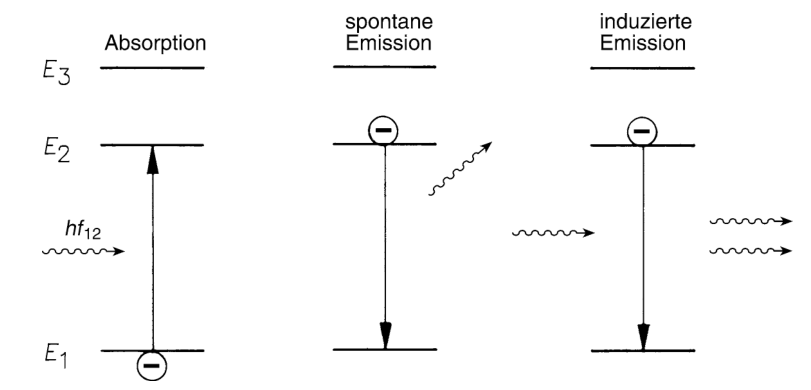
\includegraphics[width = 0.78\textwidth]{pics/Emission.png}
    \caption{Absorption, spontane Emission und induzierte Emission in einem zwei Niveau System.\cite{Laser}}
    \label{pic:emis}
\end{figure}
Für das Lasing bzw. die Verstärkung muss die Absorption kleiner sein als die induzierte Emission. Daher ist es notwendig eine Besetzungsinversion im System vorliegen zu haben.
Dies ist in einem zwei Nivea System nicht möglich, da die Zustände im thermischen Gleichgewicht der Maxwell-Boltzmann-Verteilung genügen müssen und 
somit der Grundzustand häufiger oder maximal gleich besetzt ist. Die Verstärkung nimmt exponentiell mit der Länge des Laufweges im aktiven
Lasermedium zu.
\FloatBarrier

\subsection{Helium-Neon}
Bei dem He-Ne-Laser wird ein Gasgemisch aus Helium und Neon im Verhältniss $5:1$ im aktiven Medium verwendet.
Dabei sind die Energielevel von Helium und Neon in Abbildung \ref{pic:hene} aufgezeigt. 
\begin{figure}
    \centering
    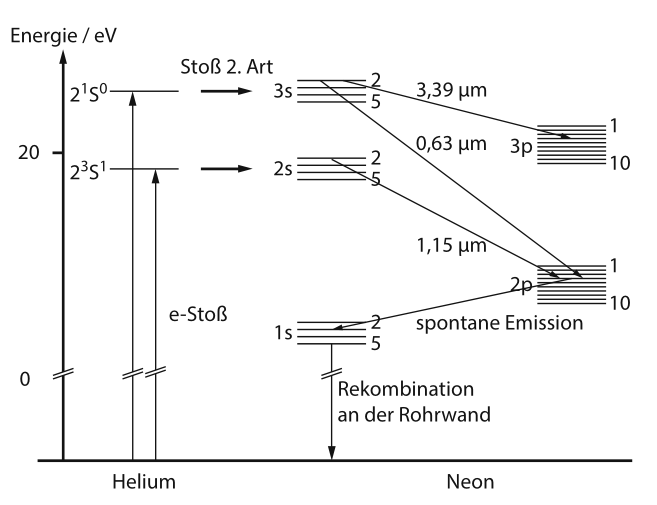
\includegraphics[width = 0.78\textwidth]{pics/HE-Ne_Termshema.png}
    \caption{Termschema des He-Ne-Lasers.\cite{Laser}}
    \label{pic:hene}
\end{figure}
Durch elektrische Entladungen wird dem System Energie zugeführt.
Dies führt zu Anregungen der Helium-Atome, welche durch Stöße 2.Art Energie an die Neon-Atome abgeben.
Dabei wird die Anregungsenergie und auch kinetische Energie übertragen.
Da der $3s$-Zustand des Heliums und der $3s_2$-Zustand des Neons ähnliche Energien haben, sind die Energieüberträge dieser Stöße resonant.
Induziert werden typische Wellenlängen des He-Ne-Lasers, wie $\SI{633}{\nano\meter}$ (Übergang $3s_2$ auf $2p_4$) und $\SI{1153}{\nano\meter}$ (Übergang $3s_2$ auf $2p_4$).
Danach kommt es zu spontaner Emission oder Rekombination an der Rohrwand, sodass sich das Elektron wieder im Grundzustand befindet.

\subsection{Resonator}
Durch einen Resonator lässt sich der Laufweg im aktiven Medium erhöhen. Wesentliche Bestandteile sind zwei Spiegel, die sich gegenüber stehen.
Einer der Spiegel sollte möglichst gut reflektieren, während der andere teils durchlässig ist und somit den Laserstrahl auskoppelt.
Der Resonator kann aus zwei planparallelen Spiegeln, zwei sphärischen Spiegeln oder aus Kombinationen der beiden Spiegeln aufgebaut sein.
Ein stabiler Resonator erfüllt die Stabilitätsbedingung
\begin{equation}
    0 < g_1 g_2 < 1 \; \text{oder} \; g_1 = g_2 = 0 \text{,}
    \label{eqn:stabi}
\end{equation}
wobei die Stabilitätsparameter $g_i$ als
\begin{equation}
    g_i = 1 - \frac{d}{b_i}
    \label{eqn:Stabilitätsparameter}
\end{equation}
definiert sind, mit der Resonatorlänge $d$ und dem Spiegelradius $b_i$.
Metastabile Zustände sind bei $g_1 g_2 = 1$ und $g_1 g_2 = 0$, dort fallen die Spiegelbrennpunkte genau zusammen.

\subsection{Räumliche Modenstrukturen}
\subsubsection{Longitudiale Moden}
Aufgrund der kleinen Wellenlängen in Relation zu den groben Aufbauten
kann nicht auf die Resonanzbedingungen geachtet werden.
Die kleinen Wellenlängen des Lichtes verhindern das einfache Einstellen der
longitudinalen Moden. Die Frequenzresonanzen entstehen in einem Abstand von
\begin{equation}
    \symup{\Delta}\nu = \frac{c}{2 n L} \, \text{,}
    \label{eqn:delnu}
\end{equation}
wobei $n$ die Anzahl der Durchläufe ist bis der Lichtstrahl wieder bei gleicher Phase am selben Ort ist.
Die Peaks sind unter einer einhüllenden Gaußkurve verstärkt, welche in Abbildung \ref{pic:kamm} zu sehen ist. 
\begin{figure}
    \centering
    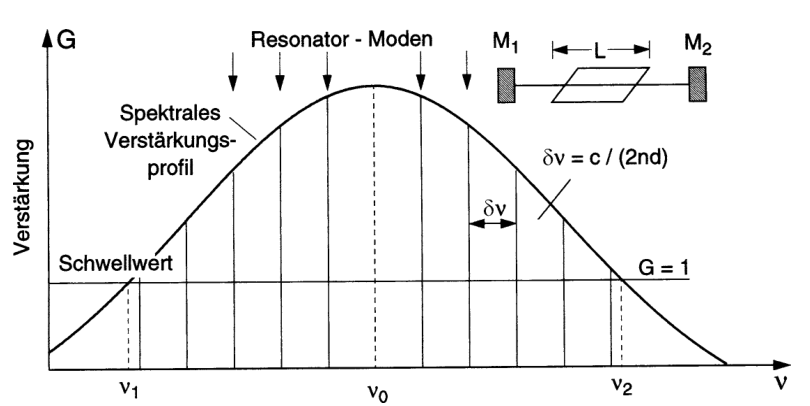
\includegraphics[width = 0.78\textwidth]{pics/kamm.png}
    \caption{Schematische Darstellung von longitudinalen Lasermoden mit einhüllender Gaußkurve.\cite{Laserspektroskopie}}
    \label{pic:kamm}
\end{figure}
Diese sogenannte Gaußverbreiterung ist ein Nebeneffekt der statistischen verteilten,
relativen Bewegungsrichtungen der Gasmoleküle im He-Ne-Plasma.
\FloatBarrier

\subsubsection{Transversale Moden}
Die transveralen Lasermoden (TEM-Moden) enstehen bei minimalen Abweichungen von der Resonatorsymmetrie.
Sie treten durch Verkippungen oder anderen Fehlern auf, da sich die Laufzeiten
der einzelnen Phononen hierdurch voneinander unterscheiden. Im stationären Betrieb
führen diese zu Interferenzen. Die Moden werden nach der Anzahl der Knoten der orthogonalen $x$-, bzw. $y$-Achse senkrecht
zur Ausbreitungsrichtung mit $\symup{TEM}_{xy}$-Moden bezeichnet. 
\begin{figure}
    \centering
    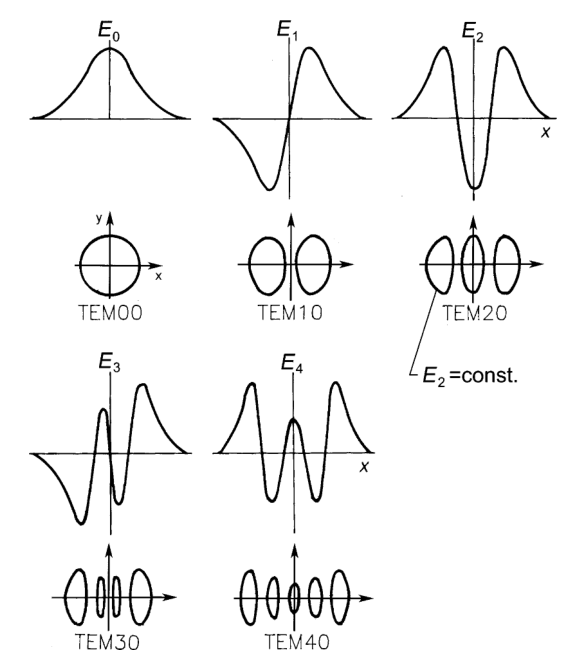
\includegraphics[width = 0.78\textwidth]{pics/Temx.png}
    \caption{Schematische Darstellung der Feldstärken-und Intensitätsverteilungen von einigen $\symup{TEM}_{x0}$-Moden.\cite{Laser}}
    \label{pic:Tem}
\end{figure}
Einige $\symup{TEM}_{x0}$-Moden sind als Feldstärkenverteilung und Intensitätsverteilung in Abbildung \ref{pic:Tem} zu sehen.
Die Feldverteilung der transversalen Moden eines konfokalen Resonators ist gegeben durch
\begin{equation}
    E_{xy}(x) \propto H_x(x) H_y(x) \symup{e}^{-\frac{x^2}{2}} \, \text{,}
\end{equation}
wobei $H_i(x)$ die Hermite-Gauß-Polynome sind. Die Intensität ist gegeben durch $I_{xy} \propto |E_{xy}(x)|^2$,
womit
\begin{equation}
    I_{xy} \propto I_0 |H_x(x) H_y(x) \symup{e}^{-\frac{x^2}{2}}|^2 
\end{equation}
folgt. Die höheren Moden haben aufgrund der geringeren Symmetrie größere Verluste.
Die Grundmode  mit den geringsten Verlusten, die $\symup{TEM}_{00}$, hat eine gaußverteilte Intensität
\begin{equation}
    I(r) = I_0 \symup{e}^{-\frac{2r^2}{\omega^2}} \, \text{,}
    \label{eqn:tem00}
\end{equation}
wobei $r$ der Abstand zur optischen Achse, $I_0$ die Maximalintensität
und $\omega(z) = \omega_0 \sqrt{1+(\frac{\omega z}{\omega_0})^2}$ der Strahlradius mit der Strahldivergenz $\omega = (\frac{\lambda}{\pi}) \omega_0$ ist.
\FloatBarrier

\subsection{Interferenz}
Kohärentes Licht, welches durch einen Spalt bzw. mehrere Spalten der Breite $b \approx \lambda$, Strahlt erzeugt Interferenzmuster.
Die Wellenlänge eines Gitters mit der Gitterkonstante $g$ lässt sich mit der Formel
\begin{equation}
    \lambda = \frac{\sin(\tan(\frac{d_k}{L}))}{g k}
    \label{eqn:gitter}
\end{equation}
berechnen. Dabei ist $d_k$ der Abstand des $k$-ten von dem $0$-ten Maximum und $L$ der Abstand vom Gitter zum Schirm.

\subsection{Polarisation}
Die Polarisationsrichtungen des durch das Brewsterfenster polarisierten Lichts kann mit Hilfe eines Polarisators bestimmt werden.
Über den Winkel $\varphi$ zwischen Polarisator und polarisierten Lichts kann mit
\begin{equation}
    I = I_0 \cos^2(\varphi)
    \label{eqn:polar}
\end{equation}
die Polarisation des Strahles ermittelt.\cite{leifi}